\hypertarget{indice}{%
\subsection{Contenidos}\label{indice}}

\begin{itemize}
\tightlist
\item
  Qué es
\item
  Gestión de datos
\item
  Memoing
\item
  Codificación
\end{itemize}

\hypertarget{definiciones}{%
\section{Definiciones}\label{definiciones}}

\hypertarget{indefinicion}{%
\subsection{Indefinición}\label{indefinicion}}

\begin{quote}
(\ldots{}) gran parte de los análisis presentados en artículos es
esencialmente temático, pero se describe como algo distinto, como
análisis de contenido, o simplemente no se identifica como un método
particular.\\
@vaismoradi\_content\_2013 {[}p. 400{]}
\end{quote}

\hypertarget{la-investigacion-cualitativa}{%
\subsection{La investigación
cualitativa}\label{la-investigacion-cualitativa}}

\begin{quote}
Un enfoque cualitativo es uno en el que hay necesidad de interpretar los
datos a través de la identificación y, posiblemente, la codificación de
temas, conceptos, procesos, contextos, etc., con el fin de construir
explicaciones o teorías o para probar o ampliar una teoría.\\
@lewins\_using\_2007
\end{quote}

\hypertarget{analisis-contenido}{%
\subsection{Análisis de contenido}\label{analisis-contenido}}

\begin{quote}
Una técnica de investigación para la descripción {objetiva, sistemática
y cuantitativa} del contenido {manifiesto} de las comunicaciones con el
fin de interpretarlas.\\
@berelson\_content\_1952 {[}p. 18{]}
\end{quote}

\hypertarget{analisis-cualitativo-contenido}{%
\subsection{Análisis cualitativo de
contenido}\label{analisis-cualitativo-contenido}}

\begin{quote}
(\ldots{}) un enfoque de análisis empírico, metodológicamente
{controlado}, de textos en su contexto de comunicación, siguiendo reglas
de análisis de contenido y modelos paso a paso, {sin una cuantificación
precipitada}.\\
@mayring\_qualitative\_2000 {[}para. 5{]}
\end{quote}

\hypertarget{analisis-tematico}{%
\subsection{Análisis temático}\label{analisis-tematico}}

\begin{quote}
El análisis temático es un método para identificar, analizar y reportar
patrones (temas) dentro de los datos. Como mínimo {organiza y describe}
en detalle el conjunto de datos. Sin embargo, con frecuencia, va más
allá e {interpreta} diversos aspectos del tema de investigación.\\
@braun\_using\_2006 {[}p. 79{]}
\end{quote}

\hypertarget{contenido-tematico}{%
\subsection{Contenido - Temático}\label{contenido-tematico}}

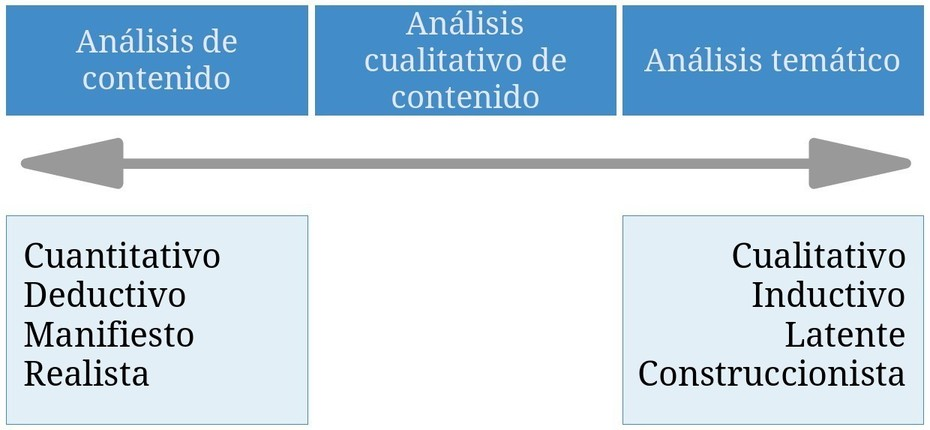
\includegraphics{imagenes-cuali/ContenidoTematico.jpg}

\hypertarget{manifiesto-latente}{%
\subsection{Manifiesto vs.~latente}\label{manifiesto-latente}}

\begin{figure}
\centering
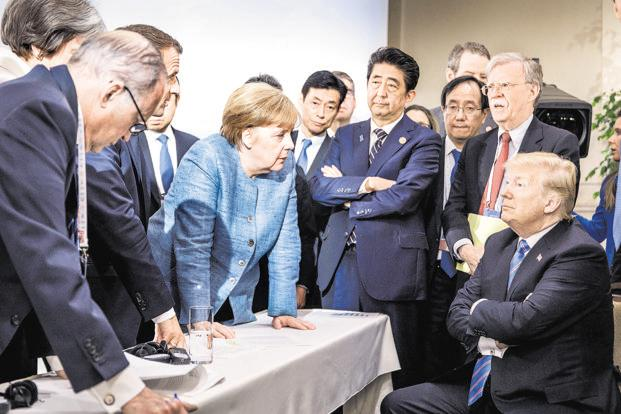
\includegraphics{imagenes-cuali/merkel-trump-merkel.jpg}
\caption{Cumbre del G7, 9 de junio de 2018, Quebec (Canadá)}
\end{figure}

Reunión del G7 en Canadá 9 junio 2018 Angel Merkel Donald Trump Justin
Trudeau Emmanuel Macron Shinzō Abe

\hypertarget{fases-analisis}{%
\subsection{Fases del análisis}\label{fases-analisis}}

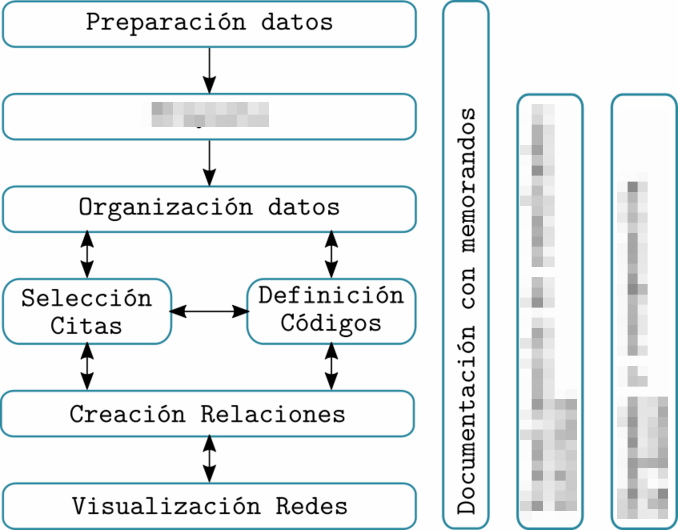
\includegraphics{imagenes-cuali/Fases.png}

\hypertarget{preparacion-datos}{%
\section{Preparación de datos}\label{preparacion-datos}}

\hypertarget{fases-preparacion-datos}{%
\subsection{Fases preparación datos}\label{fases-preparacion-datos}}

\begin{itemize}
\tightlist
\item
  Transcripción (literal de los datos)
\item
  Convenciones (``jeffersonianas'')
\item
  Gestión (archivado, formato, control)
\end{itemize}

\hypertarget{transcribir-herramientas}{%
\subsection{Transcribir: herramientas}\label{transcribir-herramientas}}

\begin{columns}[T]
\begin{column}{0.5\textwidth}
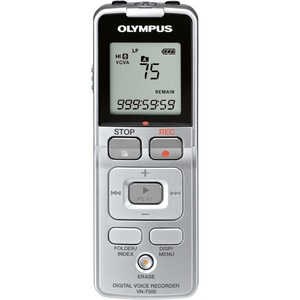
\includegraphics{imagenes-cuali/Grabadora.jpg}
\end{column}

\begin{column}{0.5\textwidth}
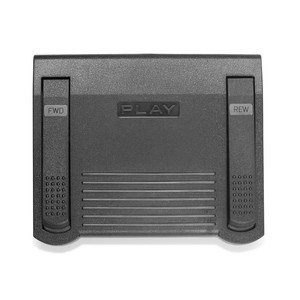
\includegraphics{imagenes-cuali/Pedal.jpg}
\end{column}
\end{columns}

\textbf{Software}

Soundscriber: \url{http://www-personal.umich.edu/~ebreck/sscriber.html}

F4: \url{http://www.audiotranskription.de/english}

\hypertarget{section}{%
\subsection{}\label{section}}

https://otranscribe.com/

\hypertarget{transcripciuxf3n-automuxe1tica}{%
\subsection{Transcripción
``automática''}\label{transcripciuxf3n-automuxe1tica}}

\begin{figure}
\centering

\includegraphics{imagenes-cuali/docs.png}
\caption{\href{https://docs.google.com/document/u/0/}{Google Docs}}
\end{figure}

\hypertarget{transcripcion}{%
\subsection{Transcripción}\label{transcripcion}}

. . .

\begin{quote}
(\ldots{}) La producción y el uso de transcripciones son {`actividades
de investigación'} y no deben ser enfocadas como simplemente `detalles
técnicos' que preceden el análisis.\\
@mclellan\_beyond\_2003 {[}p. 64{]}
\end{quote}

\hypertarget{transcripcion-realidad}{%
\subsection{Transcripción y ¿realidad?}\label{transcripcion-realidad}}

\begin{quote}
Cualquier persona que transcriba o trabaje con transcripciones debería
ser consciente de que {una transcripción nunca podrá representar una
situación de entrevista en su totalidad}. En la comunicación intervienen
demasiados elementos y es imposible transcribirlos todos. Incluso una
transcripción fonética ignora aspectos no verbales como el olor,
configuración de espacio y tiempo, aspectos visuales, expresiones
faciales y gestos.\\
@dresing\_manual\_2015 {[}p. 22{]}
\end{quote}

\hypertarget{realidad}{%
\subsection{¿Realidad?}\label{realidad}}

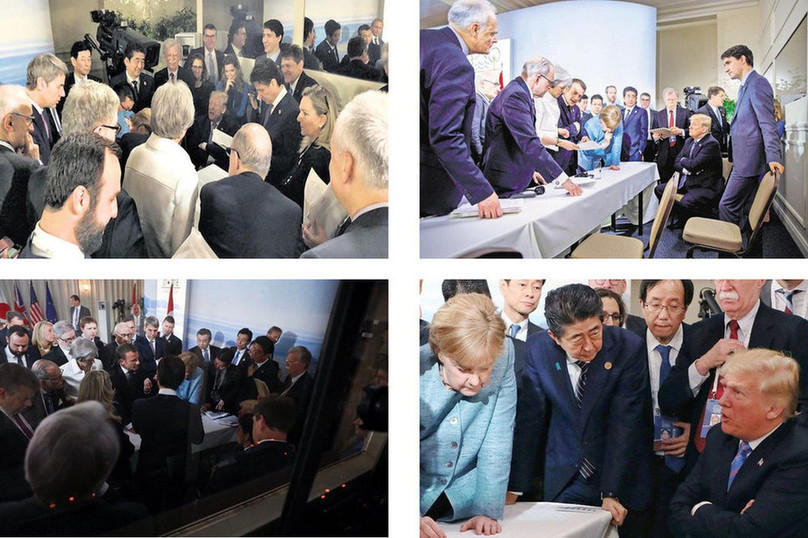
\includegraphics{imagenes-cuali/merkel-trump-otros.jpg}

\hypertarget{convenciones}{%
\subsection{Convenciones}\label{convenciones}}

\begin{quote}
En una conversación {lo más significativo es lo que no se dice entre lo
que se está diciendo}, como por ejemplo las pausas y silencios, las
entonaciones y los gestos, porque ahí radican los dobles significados,
los ánimos y el objetivo mismo de la comunicación.\\
@fernandez\_christlieb\_espiritu\_2004 {[}p. 46{]}
\end{quote}

\hypertarget{convenciones-jeffersonianas}{%
\subsection{Convenciones
``jeffersonianas''}\label{convenciones-jeffersonianas}}

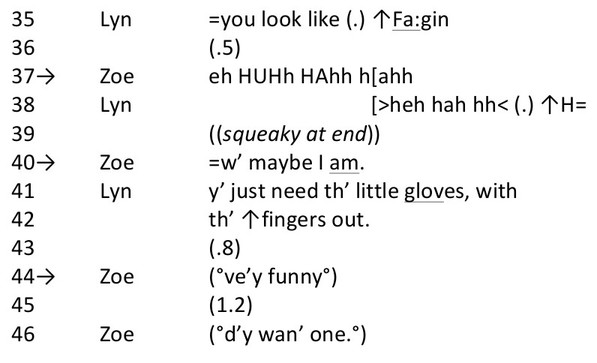
\includegraphics{imagenes-cuali/Transcripcion.jpg}

@lerner\_glossary\_2004 {[}p. 15{]}
\href{https://www.dropbox.com/s/q0sardadq3ijqsa/JeffersonianTranscriptionNotationCast.pdf?dl=0}{\textgreater{}}

Ver también: @bassi\_follari\_codigo\_2015

\hypertarget{gestion-datos-1}{%
\subsection{Gestión de los datos}\label{gestion-datos-1}}

\begin{quote}
La inadecuada documentación y monitorización de las actividades
relacionadas con los datos pueden {amenazar su integridad}. Además, las
prácticas inadecuadas de seguimiento pueden dificultar el análisis y
aumentar la probabilidad de un {pandemónium} de investigación.\\
@mclellan\_beyond\_2003 {[}p. 69{]}
\end{quote}

\href{http://www.fsd.uta.fi/aineistonhallinta/en/processing-qualitative-data-files.html}{Processing
Qualitative Data Files}\\
\texttt{http://www.fsd.uta.fi/aineistonhallinta/en/processing-qualitative-data-files.html}

\href{http://www.data-archive.ac.uk/create-manage}{UK · Data Archive:
Create \& Manage Data}\\
\texttt{http://www.data-archive.ac.uk/create-manage}

\hypertarget{plan-gestion-datos}{%
\subsection{Plan de Gestión de Datos}\label{plan-gestion-datos}}

\begin{figure}
\centering
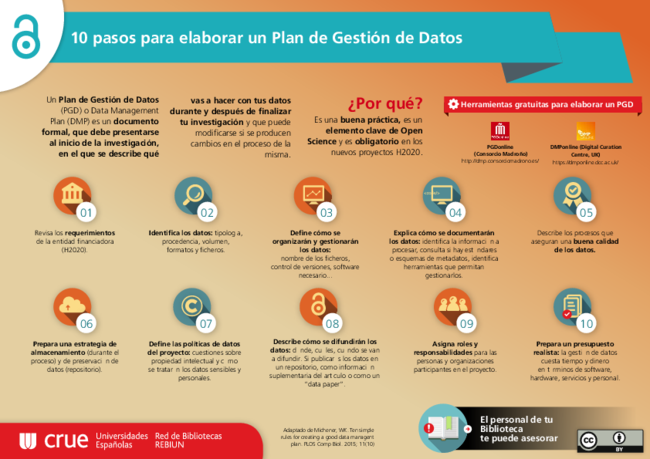
\includegraphics[width=6.77083in,height=\textheight]{imagenes-cuali/PlanDeDatos.png}
\caption{\href{http://rebiun.xercode.es/xmlui/bitstream/handle/20.500.11967/71/ES_IIIPE_Linea2_SubgOA_Info9_resolucionmedia_2016.jpg?sequence=8\&isAllowed=y}{Plan
de Gestión de Datos}}
\end{figure}

\hypertarget{dmp-csuc}{%
\subsection{}\label{dmp-csuc}}

\begin{figure}
\centering
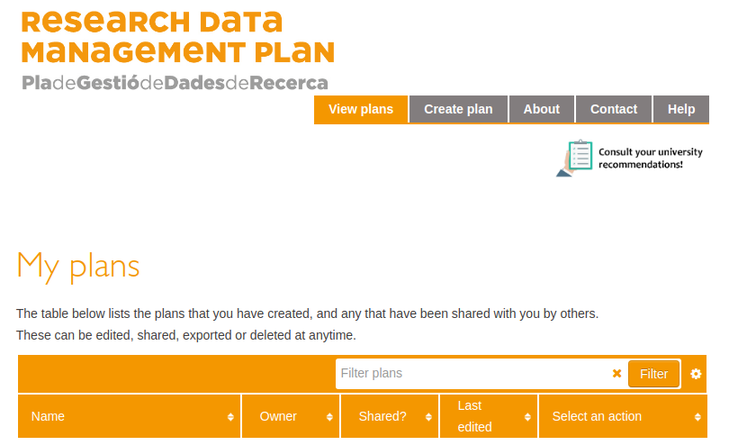
\includegraphics{imagenes-cuali/DMP-CSUC.png}
\caption{Pla de Gestió de Dades de Recerca:\\
\href{https://dmp.csuc.cat/}{https://dmp.csuc.cat}}
\end{figure}

\hypertarget{control-versiones}{%
\subsection{Control de versiones}\label{control-versiones}}

\begin{figure}
\centering
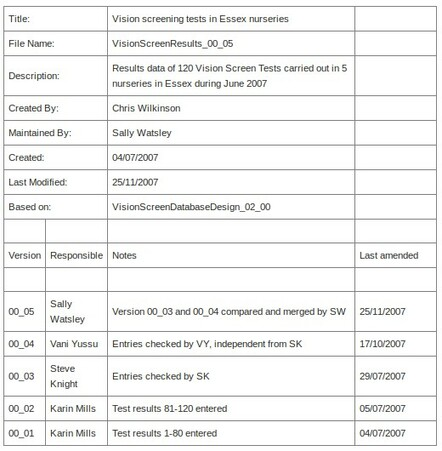
\includegraphics{imagenes-cuali/VersionControlTable.jpg}
\caption{\url{https://www.ukdataservice.ac.uk/manage-data/format/versioning}}
\end{figure}

\hypertarget{ejercicio-gestion}{%
\subsection{Ejercicio: Gestión de datos}\label{ejercicio-gestion}}

\leavevmode\hypertarget{column2}{}%

\includegraphics{img/GroupWork.jpg}

\hypertarget{column2}{}
\begin{quote}
\begin{itemize}
\tightlist
\item
  Formato documentos
\item
  Etiquetado archivos
\item
  Sistema de control
\item
  \ldots{}
\end{itemize}
\end{quote}

\hypertarget{y-luego}{%
\subsection{Y luego\ldots{}}\label{y-luego}}

. . .

\begin{figure}
\centering

\includegraphics{imagenes-cuali/reader-4.png}
\caption{para después\ldots{}}
\end{figure}

. . .


\includegraphics{imagenes-cuali/readers.jpg}

\hypertarget{memoing-1}{%
\section{Memoing}\label{memoing-1}}

\hypertarget{memoing-3}{%
\subsection{Memoing}\label{memoing-3}}

\begin{quote}
Vemos la toma de notas como {crucial} para todos los tipos y enfoques de
análisis. Otras funciones, como la codificación, la búsqueda de texto,
la codificación automática y la modelización pueden ser utilizadas por
enfoques concretos, pero la anotación de los datos, documentos y
material de apoyo es {indivisible del análisis general}.\\
@lewins\_using\_2007 {[}p. 59{]}
\end{quote}

\hypertarget{memoing-reflexionar}{%
\subsection{Memoing = Reflexionar
sobre\ldots{}}\label{memoing-reflexionar}}

\begin{quote}
\begin{itemize}
\tightlist
\item
  Relación con participantes y/o fenómeno
\item
  Preguntas de investigación
\item
  Elección de códigos y sus definiciones
\item
  Categorías, temas y conceptos emergentes
\item
  Posibles conexiones entre elementos
\item
  Teoría emergente
\item
  Problemas de cualquier tipo de nuestra investigación
\item
  Problemas o dilemas éticos
\item
  Informe final
\end{itemize}
\end{quote}

@saldana\_coding\_2009 {[}pp. 34-40{]}

\hypertarget{codificacion}{%
\section{Codificación}\label{codificacion}}

\hypertarget{como}{%
\subsection{¿Cómo?}\label{como}}

\begin{figure}
\centering
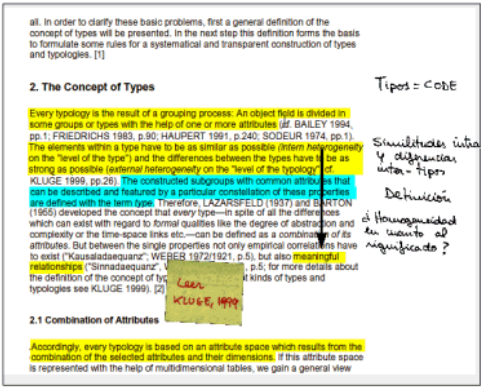
\includegraphics{imagenes-cuali/AnalisisCotidiano.png}
\caption{Análisis ``cotidiano''}
\end{figure}

\hypertarget{esquema-saldana}{%
\subsection{}\label{esquema-saldana}}

\begin{figure}
\centering
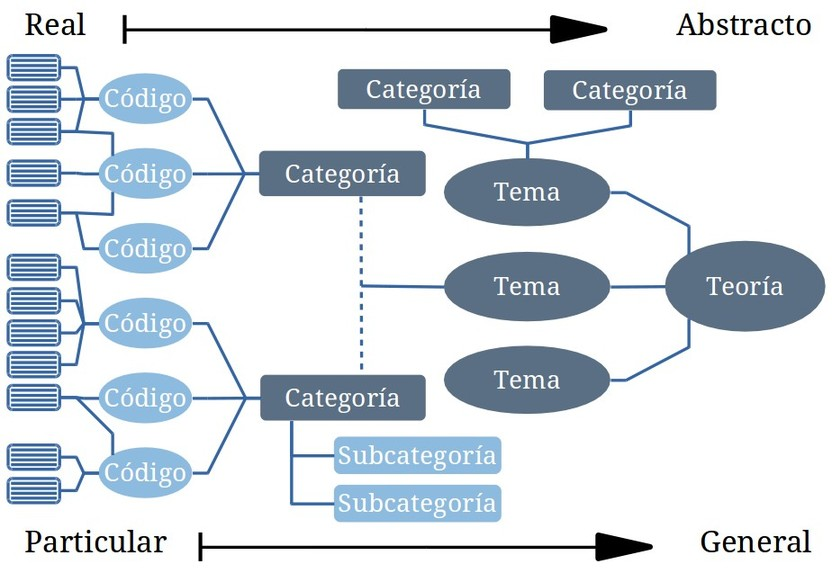
\includegraphics{imagenes-cuali/DatoATeoria.jpg}
\caption{Adaptado de Saldaña, 2009, p.~12}
\end{figure}

\hypertarget{ejemplo}{%
\subsection{Ejemplo: códigos-categorías-temas}\label{ejemplo}}

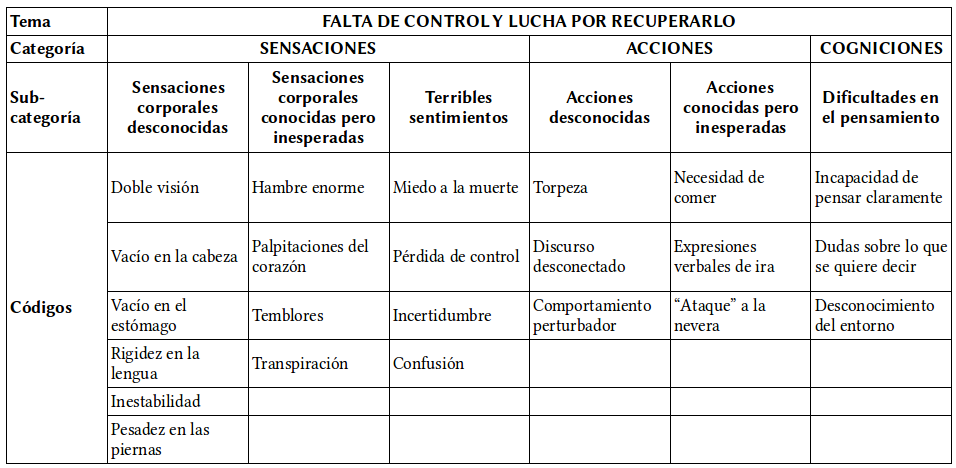
\includegraphics{imagenes-cuali/Graneheim-Lundaman-Figura1-es.png}
@graneheim\_qualitative\_2004 {[}p. 108{]}\\
\texttt{Narrativas\ sobre\ hipoglucemia}

\hypertarget{proceso-analisis}{%
\subsection{Proceso de análisis}\label{proceso-analisis}}

\begin{figure}
\centering
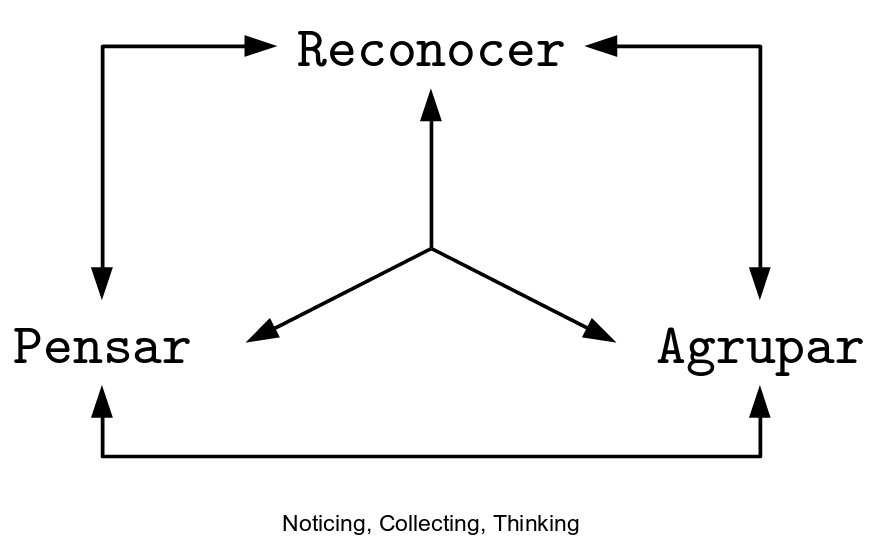
\includegraphics{imagenes-cuali/Seidel-NCT.png}
\caption{Adaptado de @seidel\_qualitative\_1998 {[}p. 2{]}}
\end{figure}

\hypertarget{reduccion}{%
\subsection{Reducción}\label{reduccion}}

\begin{quote}
{[}En la investigación cualitativa{]} el reto es dar sentido a una
cantidad masiva de datos, reducir el volumen de información, identificar
pautas significativas, y construir un marco para comunicar la esencia de
lo que revelan los datos.\\
@patton\_qualitative\_1990 {[}pp. 371-372{]}
\end{quote}

. . .

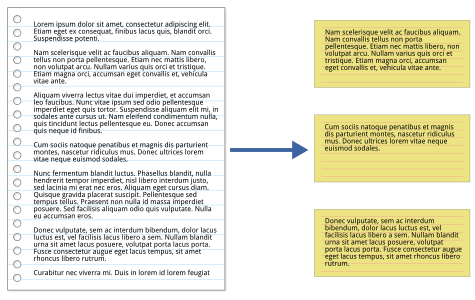
\includegraphics[width=3.64583in,height=\textheight]{imagenes-cuali/Reduccion.png}

\hypertarget{comentarios-codigos}{%
\subsection{Comentarios de códigos}\label{comentarios-codigos}}

\begin{longtable}[]{@{}ll@{}}
\toprule
\begin{minipage}[b]{0.07\columnwidth}\raggedright
Código\strut
\end{minipage} & \begin{minipage}[b]{0.87\columnwidth}\raggedright
MARGPROB\strut
\end{minipage}\tabularnewline
\midrule
\endhead
\begin{minipage}[t]{0.07\columnwidth}\raggedright
Definición breve\strut
\end{minipage} & \begin{minipage}[t]{0.87\columnwidth}\raggedright
Problemas propios de comunidades marginales\strut
\end{minipage}\tabularnewline
\begin{minipage}[t]{0.07\columnwidth}\raggedright
Definición completa\strut
\end{minipage} & \begin{minipage}[t]{0.87\columnwidth}\raggedright
Situaciones sociales que son vividas exclusivamente por aquellas
personas que llevan un estilo de vida marginal, con carencia
fundamentalmente de bienes y servicios que sí están presentes en
personas con nivel socioeconómico medio.\strut
\end{minipage}\tabularnewline
\begin{minipage}[t]{0.07\columnwidth}\raggedright
Cuándo se usa\strut
\end{minipage} & \begin{minipage}[t]{0.87\columnwidth}\raggedright
Cuando las personas señalan alguna dificultad que denote un problema
social instrumental, como falta de alimento, abrigo, techo, salud,
servicios sanitarios. Debe tener carácter grave o impedir el desarrollo
adecuado de su vida familiar, social o laboral.\strut
\end{minipage}\tabularnewline
\begin{minipage}[t]{0.07\columnwidth}\raggedright
Cuándo no se usa\strut
\end{minipage} & \begin{minipage}[t]{0.87\columnwidth}\raggedright
No se aplica a problemas propios de una conducta condicionada por
cultura marginal, como violencia doméstica, alcoholismo, abandono de
hogar, delincuencia, prostitución\strut
\end{minipage}\tabularnewline
\begin{minipage}[t]{0.07\columnwidth}\raggedright
Ejemplo\strut
\end{minipage} & \begin{minipage}[t]{0.87\columnwidth}\raggedright
``Como aquí no hay agua ni alcantarillado, la suciedad que hay aquí en
las calles es terrible, ahí se puede ver\ldots{} ¿se fija?, los niños se
enferman a cada rato.''\strut
\end{minipage}\tabularnewline
\bottomrule
\end{longtable}

@macqueen\_codebook\_1998

\hypertarget{codificacion-depuracion}{%
\subsection{Codificación:
``Depuración''}\label{codificacion-depuracion}}

\begin{quote}
Durante el desarrollo de un sistema de códigos y eventualmente temas, el
investigador va en constante ir y venir entre la lectura de los datos,
la relectura de los segmentos codificados, la organización de los
códigos, el cambio de nombre y el reordenamiento de los códigos y la
recodificación de los segmentos de datos.\\
@friese\_carrying\_2018 {[}p. 17{]}
\end{quote}

\hypertarget{comparacion-constante}{%
\subsection{Comparación constante}\label{comparacion-constante}}

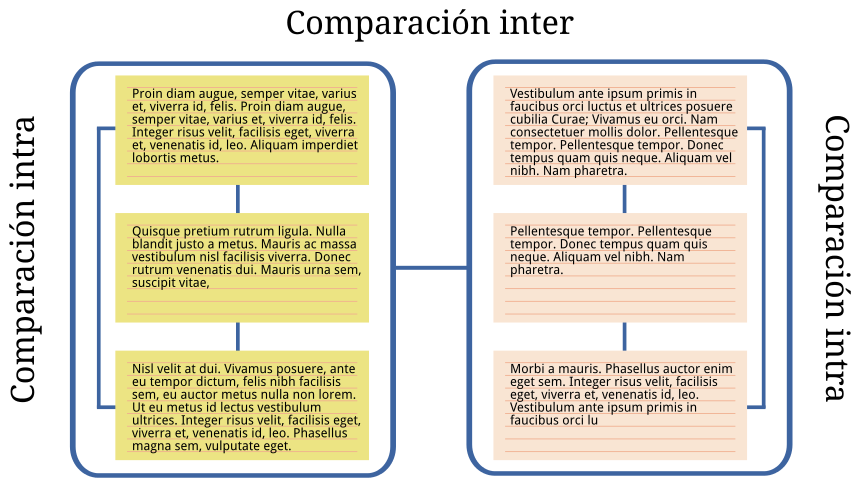
\includegraphics{imagenes-cuali/comparacion-constante.png}

\hypertarget{section-1}{%
\subsection{}\label{section-1}}

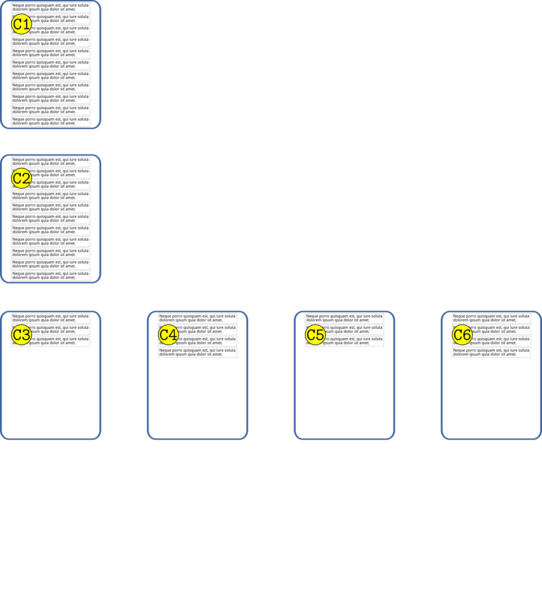
\includegraphics{imagenes-atlas-8/Categorizacion01.png}

\hypertarget{section-2}{%
\subsection{}\label{section-2}}

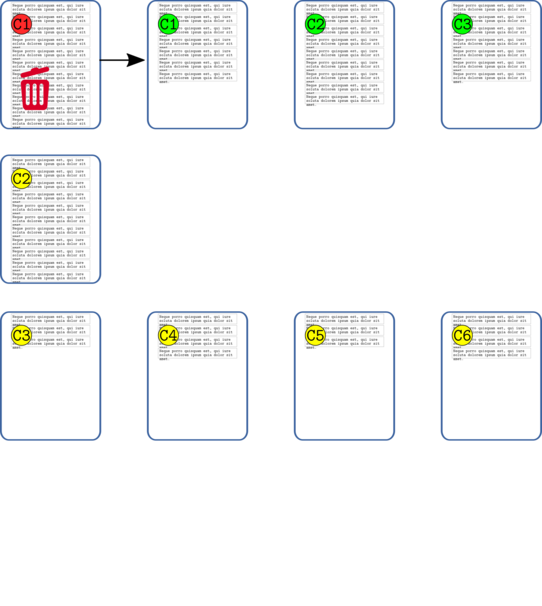
\includegraphics{imagenes-atlas-8/Categorizacion02.png}

\hypertarget{section-3}{%
\subsection{}\label{section-3}}

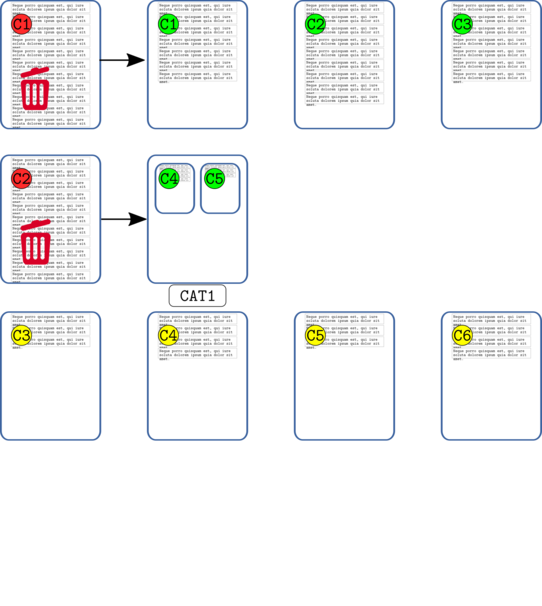
\includegraphics{imagenes-atlas-8/Categorizacion03.png}

\hypertarget{section-4}{%
\subsection{}\label{section-4}}

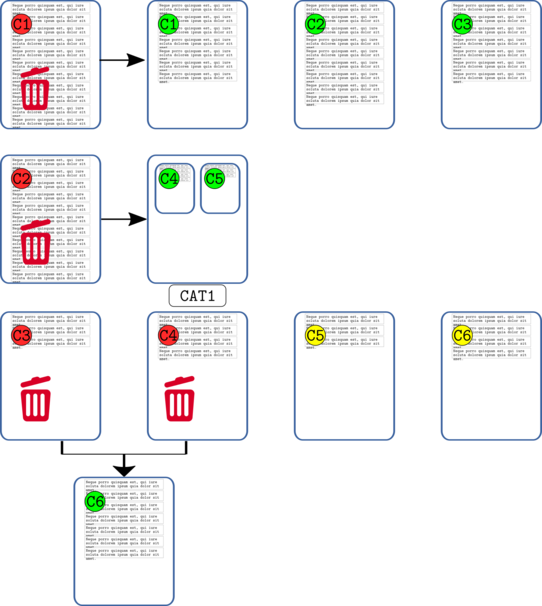
\includegraphics{imagenes-atlas-8/Categorizacion04.png}

\hypertarget{section-5}{%
\subsection{}\label{section-5}}

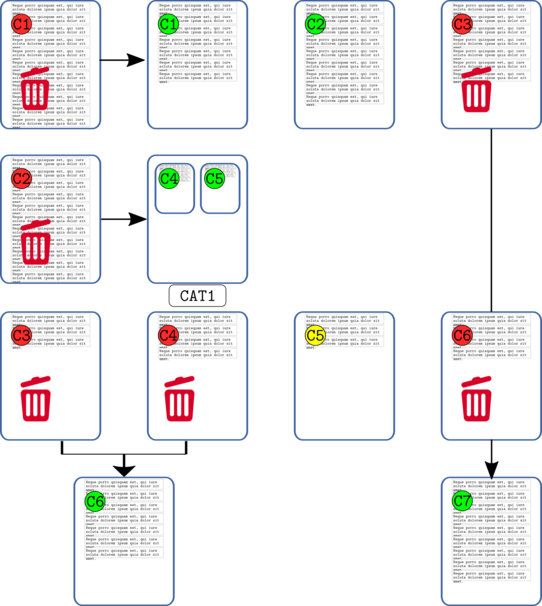
\includegraphics{imagenes-atlas-8/Categorizacion05.png}

\hypertarget{section-6}{%
\subsection{}\label{section-6}}

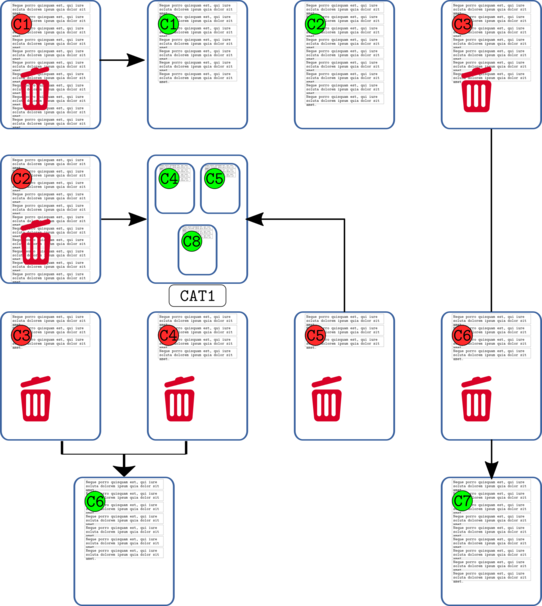
\includegraphics{imagenes-atlas-8/Categorizacion06.png}

@friese\_using\_2011

\hypertarget{temas}{%
\subsection{Temas}\label{temas}}

\begin{quote}
Un tema capta algo importante sobre los datos en relación con la
pregunta de investigación, y representa un cierto nivel de pauta de
respuesta o significado en el conjunto de los datos.\\
@braun\_using\_2006 {[}p. 82{]}
\end{quote}

\hypertarget{agrupar-relacionar}{%
\subsection{Agrupar y relacionar: Redes
temáticas}\label{agrupar-relacionar}}

\begin{quote}
Aplicar redes temáticas es simplemente una forma de organizar un
análisis temático de datos cualitativos. Los análisis temáticos intentan
descubrir los temas más destacados en un texto a diferentes niveles, y
las redes temáticas tienen como objetivo {facilitar la estructuración y
representación} de esos temas.\\
@attride-stirling\_thematic\_2001 {[}p. 387{]}
\end{quote}

\hypertarget{redes-tematicas}{%
\subsection{Redes temáticas}\label{redes-tematicas}}

\begin{figure}
\centering
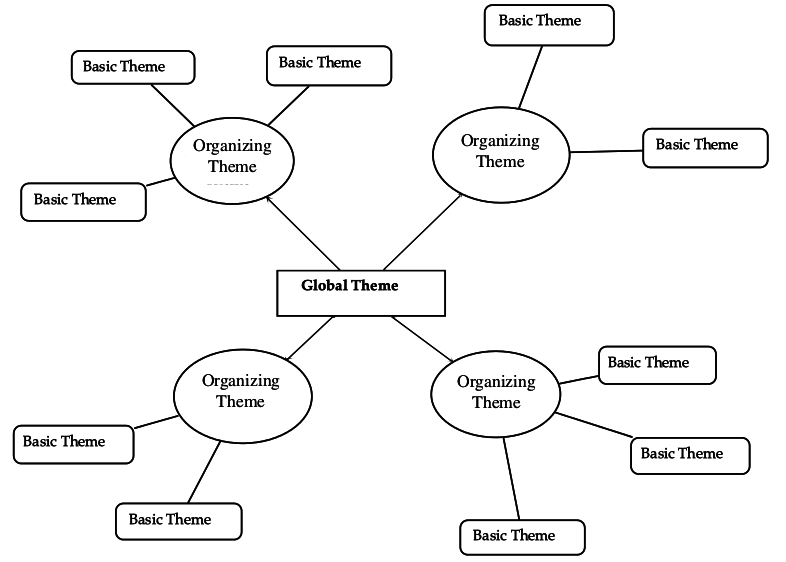
\includegraphics{imagenes-cuali/RedesTematicas.png}
\caption{Attride-Stirling, 2001. p.~388}
\end{figure}

\hypertarget{redes-tematicas-2}{%
\subsection{Redes temáticas}\label{redes-tematicas-2}}

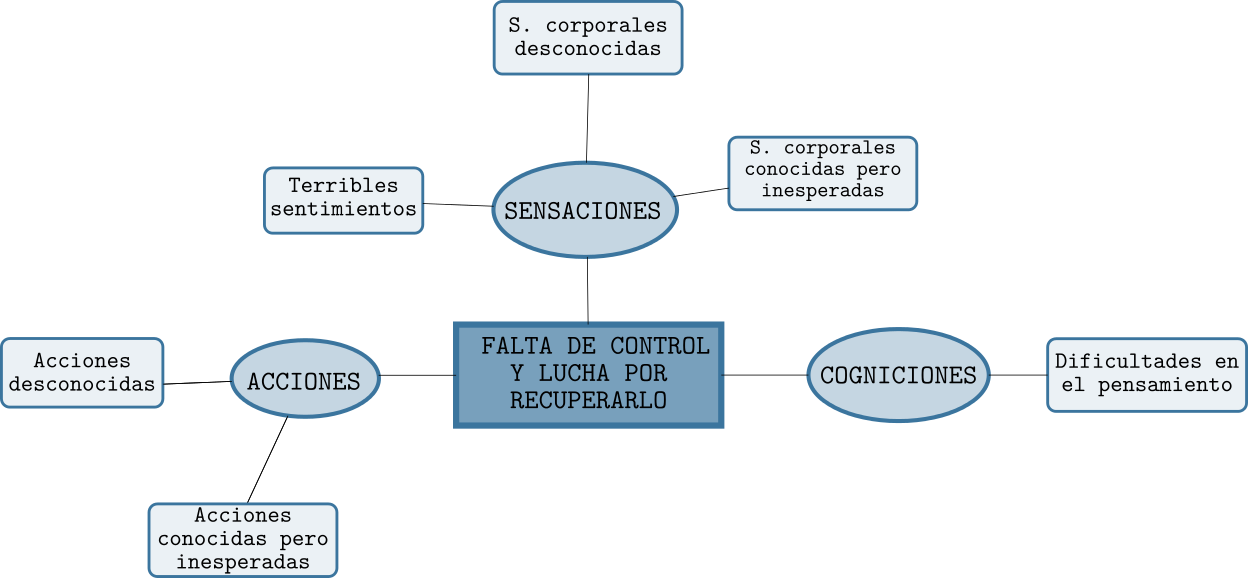
\includegraphics{imagenes-cuali/RedesTematicas-2.png}

\hypertarget{relaciones-codigos-donacion}{%
\subsection{Redes}\label{relaciones-codigos-donacion}}

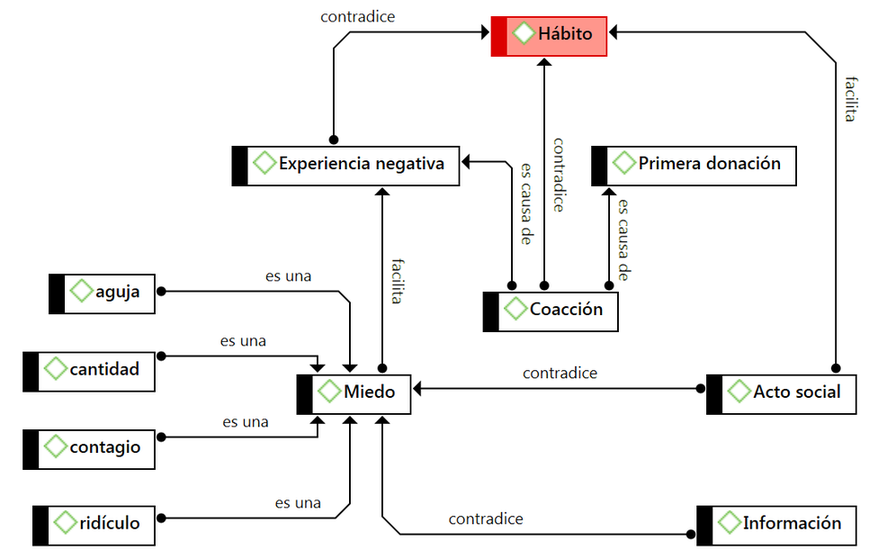
\includegraphics{imagenes-atlas-8/red-donacion.png}

\hypertarget{referencias}{%
\section{Referencias}\label{referencias}}

\hypertarget{section-7}{%
\subsection{}\label{section-7}}
